\begin{figure}[H]
	\centering
	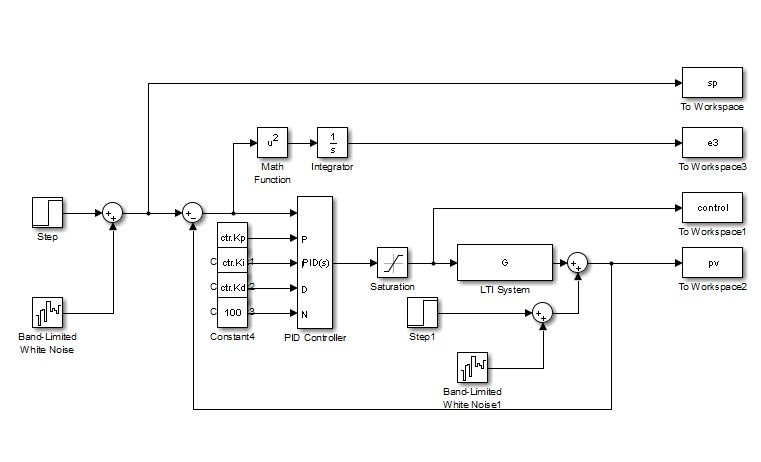
\includegraphics[width=140mm]{ClosedLoopModel.jpg}
	\caption{Model w Simulinku}
	\label{fig:model_simulink}
\end{figure}

Poniżej przedstawiono skrypt napisany w Matlabie.
\begin{lstlisting} 
quality=[];
load('transfer_functions.mat')
n=9;
m=[21 21 10 6 9 9 36 11 10];
simulation_time = 30;
model_nsat = 'PIDmodel_nsat.slx';
model_sat = 'PIDmodel_sat.slx';
model_sat_noise = 'PIDmodel_sat_noise.slx';
for i = 1:n
	for j=1:m(i)
		try
			%% Load transfer function %%
			name=strcat('G',num2str(i),'(',num2str(j),')');
			G = eval(name);
			transfer_function=strcat('$$G(s)=',latex(poly2sym(cell2mat(eval(strcat(name,'.num'))),s)
				/poly2sym(cell2mat(eval(strcat(name,'.den'))),s)),'$$');
		
			%% Plot step response %%
			fig = figure();
			h=subplot(2,1,1);
			step(G,simulation_time);
			grid on;
		
			%% Design PID controller %%
			[ctr,info]=pidtune(G,'pid');
			cmd_sys=feedback(ctr*G,1);    
		
			%% Perform simulation (not saturated), plot model response %%
			sim(model_nsat); 
			
			h=subplot(2,1,2);
			plot(sp, 'r');
			hold on;
			plot(control, 'g');
			plot(pv, 'b');
			grid on;
			ylabel('Amplitude');
			xlabel('Time (seconds)');
			title(strcat(transfer_function,', Saturation: off, Noise: off', ', e=',
			num2str(e1.Data(length(e1.Data)))), 'Interpreter', 'Latex')
			legend('set value','control value','response value', 'Location','southeast');
		
			%% Save to file 1%%
			file = strcat('sprawozdanie\G',int2str(i),'-tf-', int2str(j),'a');
			print(fig,file,'-dpng');
			close(fig)
			%% Perform simulation (saturated), plot model response %%
			sim(model_sat); 
	
			fig = figure();            
			h=subplot(2,1,1);
			plot(sp, 'r');
			hold on;
			plot(control, 'g');
			plot(pv, 'b');
			grid on;
			ylabel('Amplitude');
			xlabel('Time (seconds)');
			title(strcat(transfer_function, ', Saturation: on, Noise: off ',',
			 e=',num2str(e2.Data(length(e2.Data)))), 'Interpreter', 'Latex')
			legend('set value','control value','response value', 'Location','southeast');
	
	
	
			%% Perform simulation (saturated with noise), plot model response %%
			sim(model_sat_noise);
		
			h=subplot(2,1,2);
			plot(sp, 'r');
			hold on;
			plot(control, 'g');
			plot(pv, 'b');
			grid on;
			ylabel('Amplitude');
			xlabel('Time (seconds)');
			title(strcat(transfer_function, ', Saturation: on, Noise: on ',',
			 e=',num2str(e3.Data(length(e3.Data)))), 'Interpreter', 'Latex')
			legend('set value','control value','response value', 'Location','southeast');
	
			quality=[quality; i j e1.Data(length(e1.Data)) e2.Data(length(e2.Data)) e3.Data(length(e3.Data))];
			%% Save to file 2%%
			file = strcat('sprawozdanie\G',int2str(i),'-tf-', int2str(j),'b');
			print(fig,file,'-dpng');
			close(fig)
		catch ME
			strcat('Błąd w: G',int2str(i),'(',int2str(j),').')
		end
	end
end
save('sprawozdanie\report.txt','quality','-ascii')

\end{lstlisting}
